\begin{frame}{Podcast: Hours Rambled}
    \note{\scriptsize
Moving on, let's discuss the duration of the \emph{ÍSKISUR} podcast episodes available on Alvarpið (a free streaming platform syndicated on Nútíminn.is) and the subscription-based Storytel.

Both platforms introduced the series with a teaser. However, their approaches varied:
\begin{itemize}
    \item Alvarpið had a more freestyle format.
    \item Storytel adhered to a structured approach, ensuring uniform episode durations.
\end{itemize}

The data highlights this: Over 4 years, we produced 7,762 minutes (or 5 days) of content. Episodes on Storytel averaged just under an hour, roughly 10 minutes longer than on Alvarpið. Notably, no episode on either platform exceeded 75 minutes, underscoring our aim for concise, captivating content.
}

    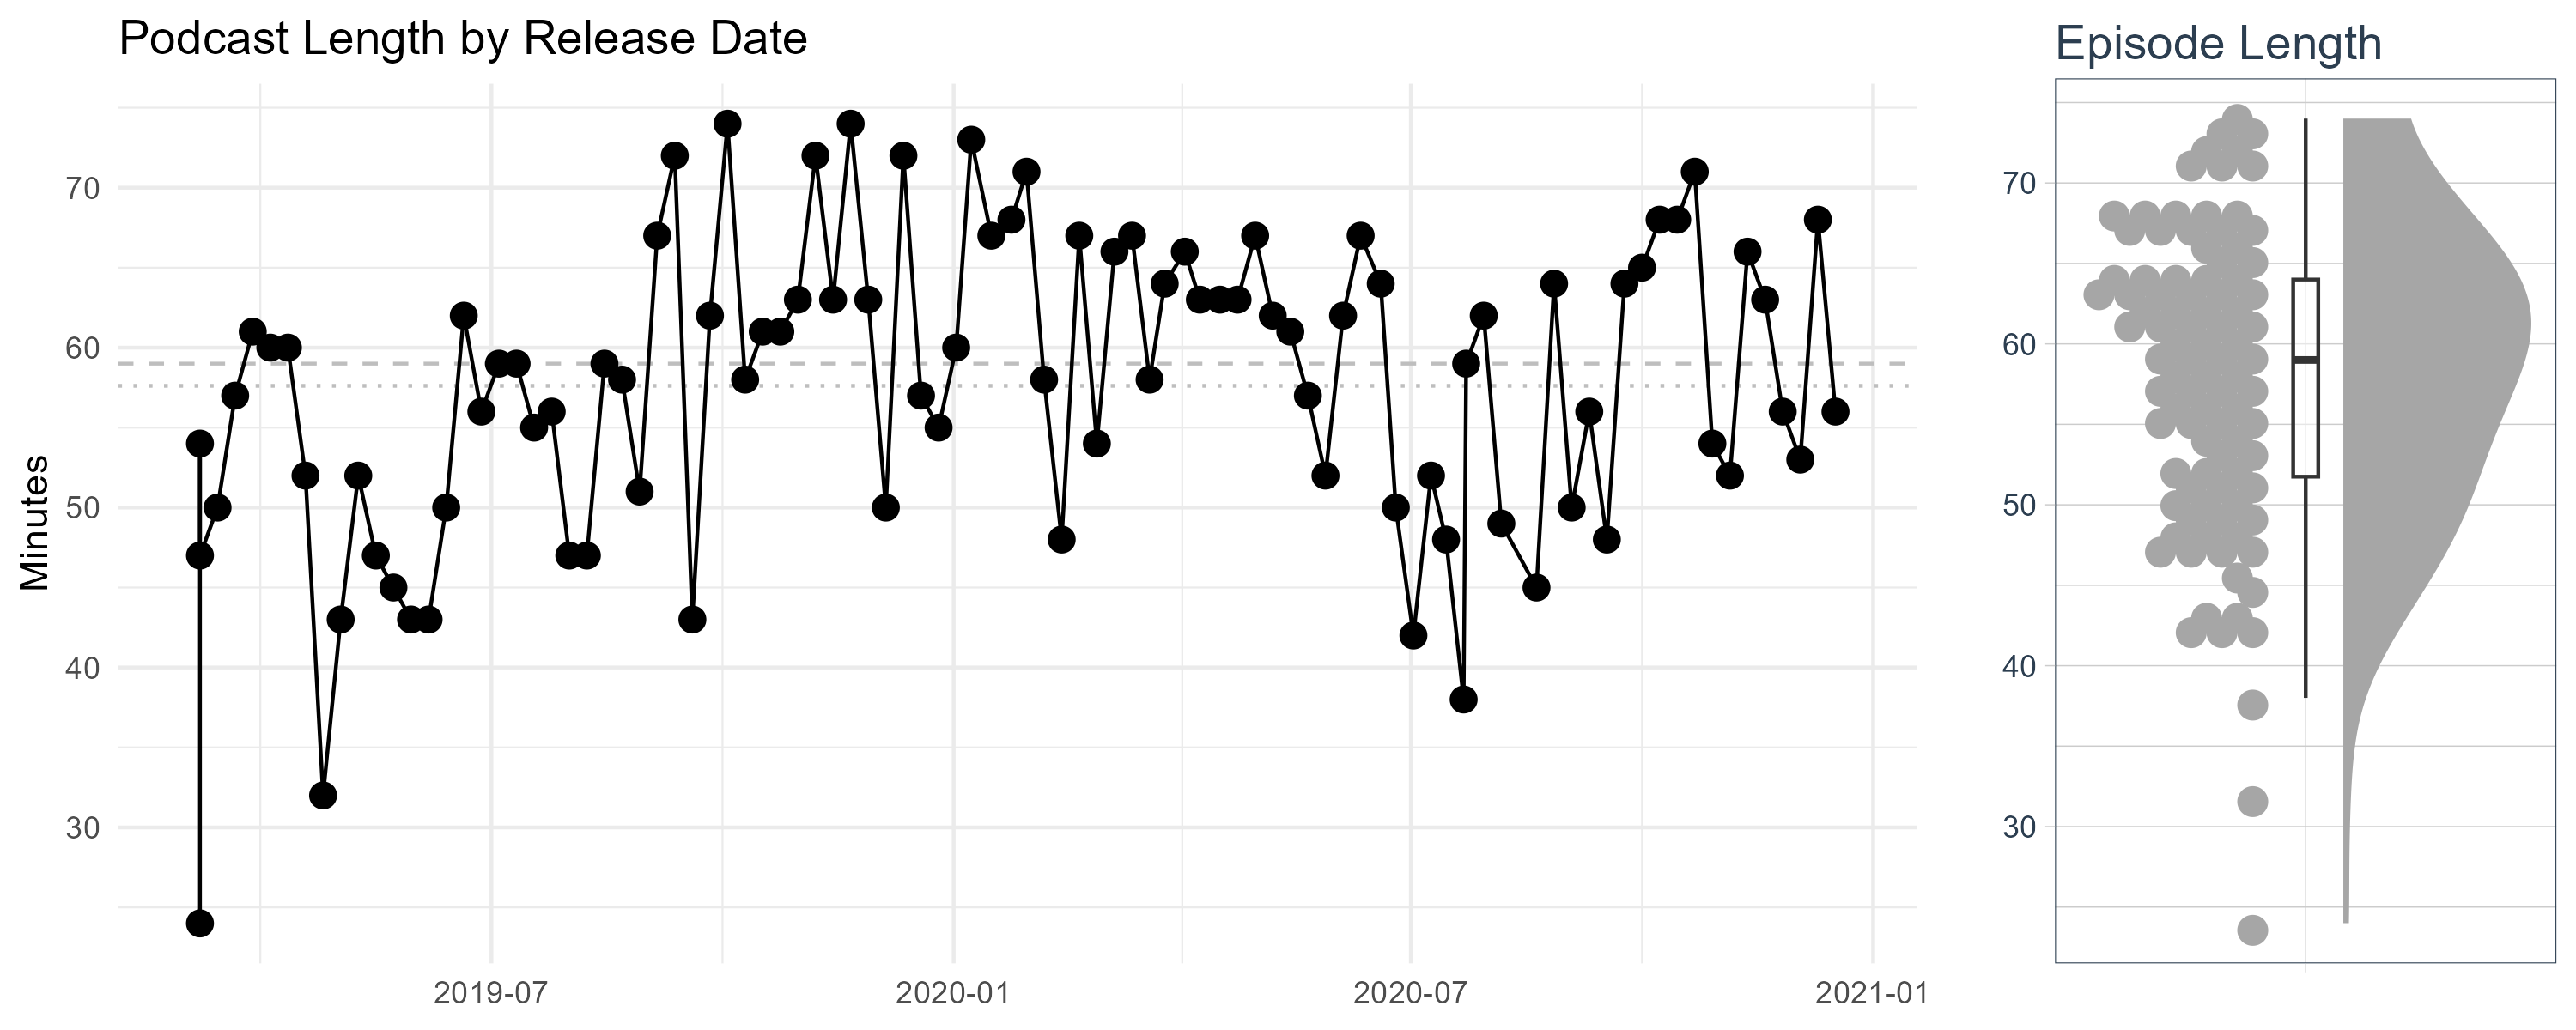
\includegraphics[width=\textwidth]{../rek-data-beers/R/figures/iskisur_length}
    \begin{itemize}
        \item Over a period of 45.8 months, there is 7,762 minutes of \emph{quality} content, or 5.4 days of continuous
        listening.
        \item Average length is 57.6 minutes on Storytel (48.5 on Alvarpið), but never surpassing 75 minutes.
    \end{itemize}
\end{frame}

\begin{frame}{Podcast on Alvarpið}
\note{
Diving into our experience with the Alvarpið platform: Over 20 months, we crafted 46 episodes, delving into 5.5 books.

\begin{itemize}
    \item Although I couldn't get exact listener counts for each episode, we were informed of a range of \emph{800-1000} listeners per episode through platforms like iTunes.
    Data from \emph{Nútíminn}, via Mixcloud, reflects around 40 streams per episode.
    \item We started with one chapter per episode but quickly transitioned to two chapters for sustainability.
    \item Challenges arose by the sixth book, with health issues and logistical obstacles cutting short our coverage.
    \item Kristín and I recorded from Reykjavík while Birna was in Reyðarfjörður, revealing the hurdles of independent production.
    \item Fortuitously, Storytel approached us. Their entry not only promised compensation but also took over technical aspects, letting us focus on book discussions and my personal favorite: the cat segment.
\end{itemize}
}
    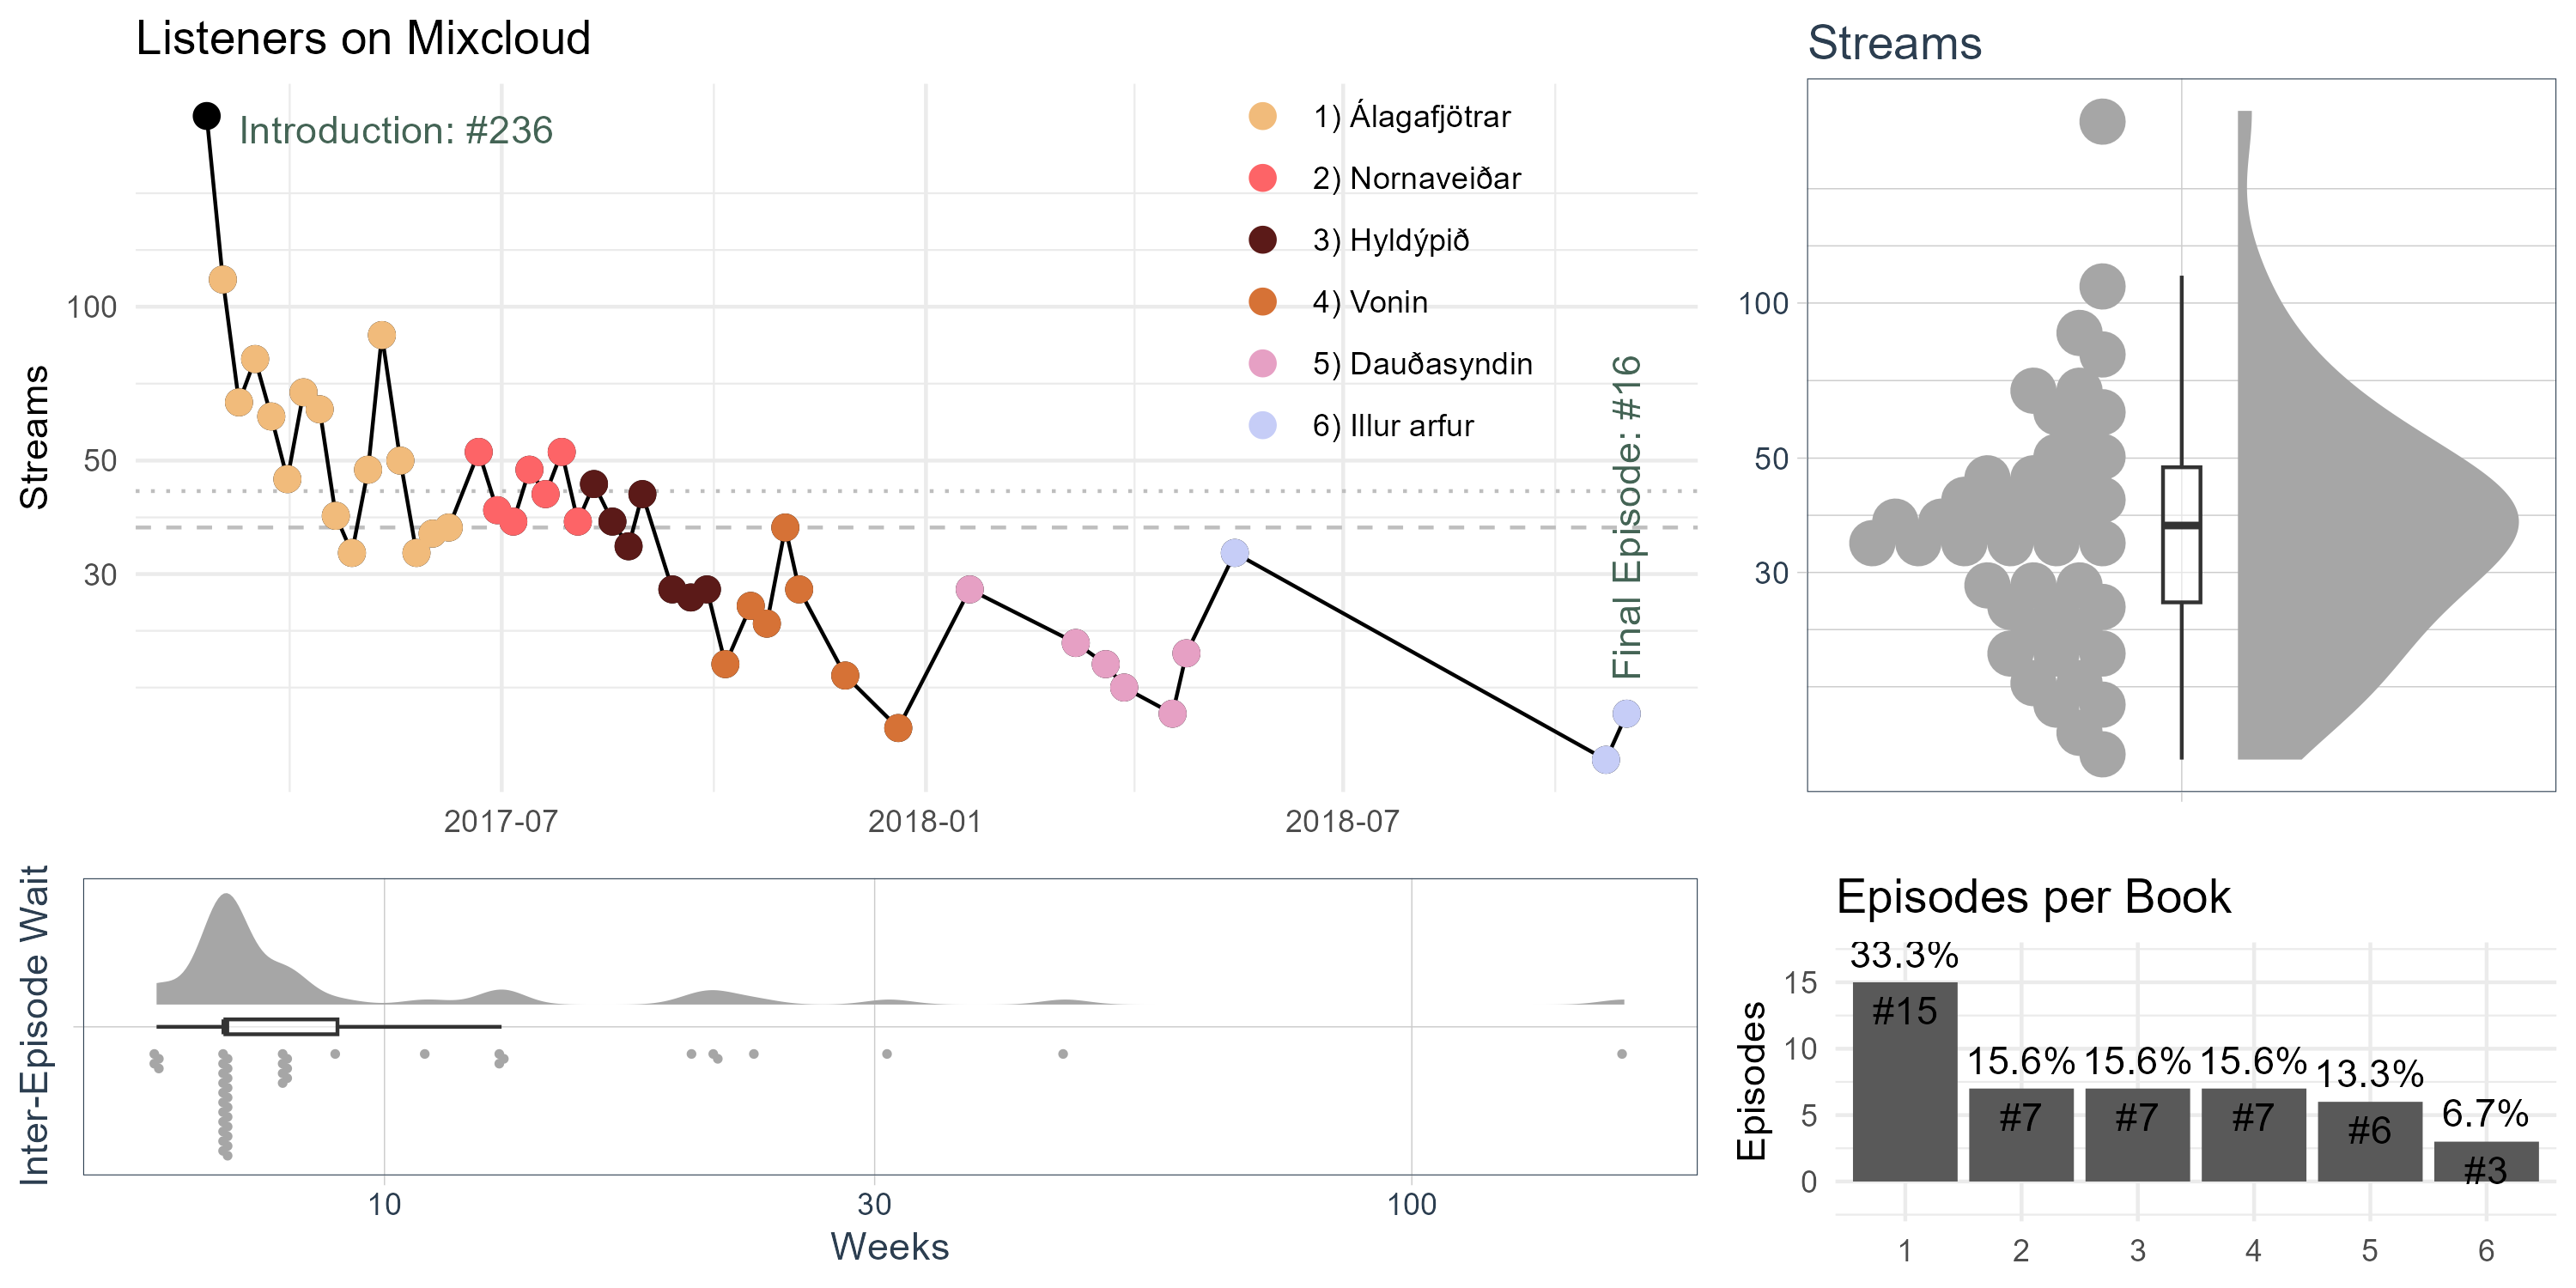
\includegraphics[width=\textwidth]{../rek-data-beers/R/figures/alvarpid_listeners}
    \vspace{-12pt}
    \begin{itemize}
        \item 46 episodes, 20 months, 5.5 books
        \item 2,231 minutes -- 37 hours -- 1.5 days of continuous listening
        \item Roughly 1,040 streams per episode (thereof ~40 via \url{nutiminn.is})
    \end{itemize}
\end{frame}

\begin{frame}{Podcast on Storytel: High Ratings}
\note{
Teaming up with Storytel brought not just technical relief but also glowing audience feedback, as depicted in this chart.
\begin{itemize}
    \item Our average rating is an outstanding 4.74 out of 5.
    \item Over half of our episodes, 54 to be exact, received a flawless score of 5.0, highlighting listener satisfaction.
    \item Only seven episodes went below a 4.0 rating, with the least score being 3.3.
    \item These figures reflect the consistent quality of our content, augmented by Storytel's professional touch.
\end{itemize}

Switching from the hurdles of Alvarpið's self-production to the streamlined process with Storytel gave our mission renewed vigor.
}
    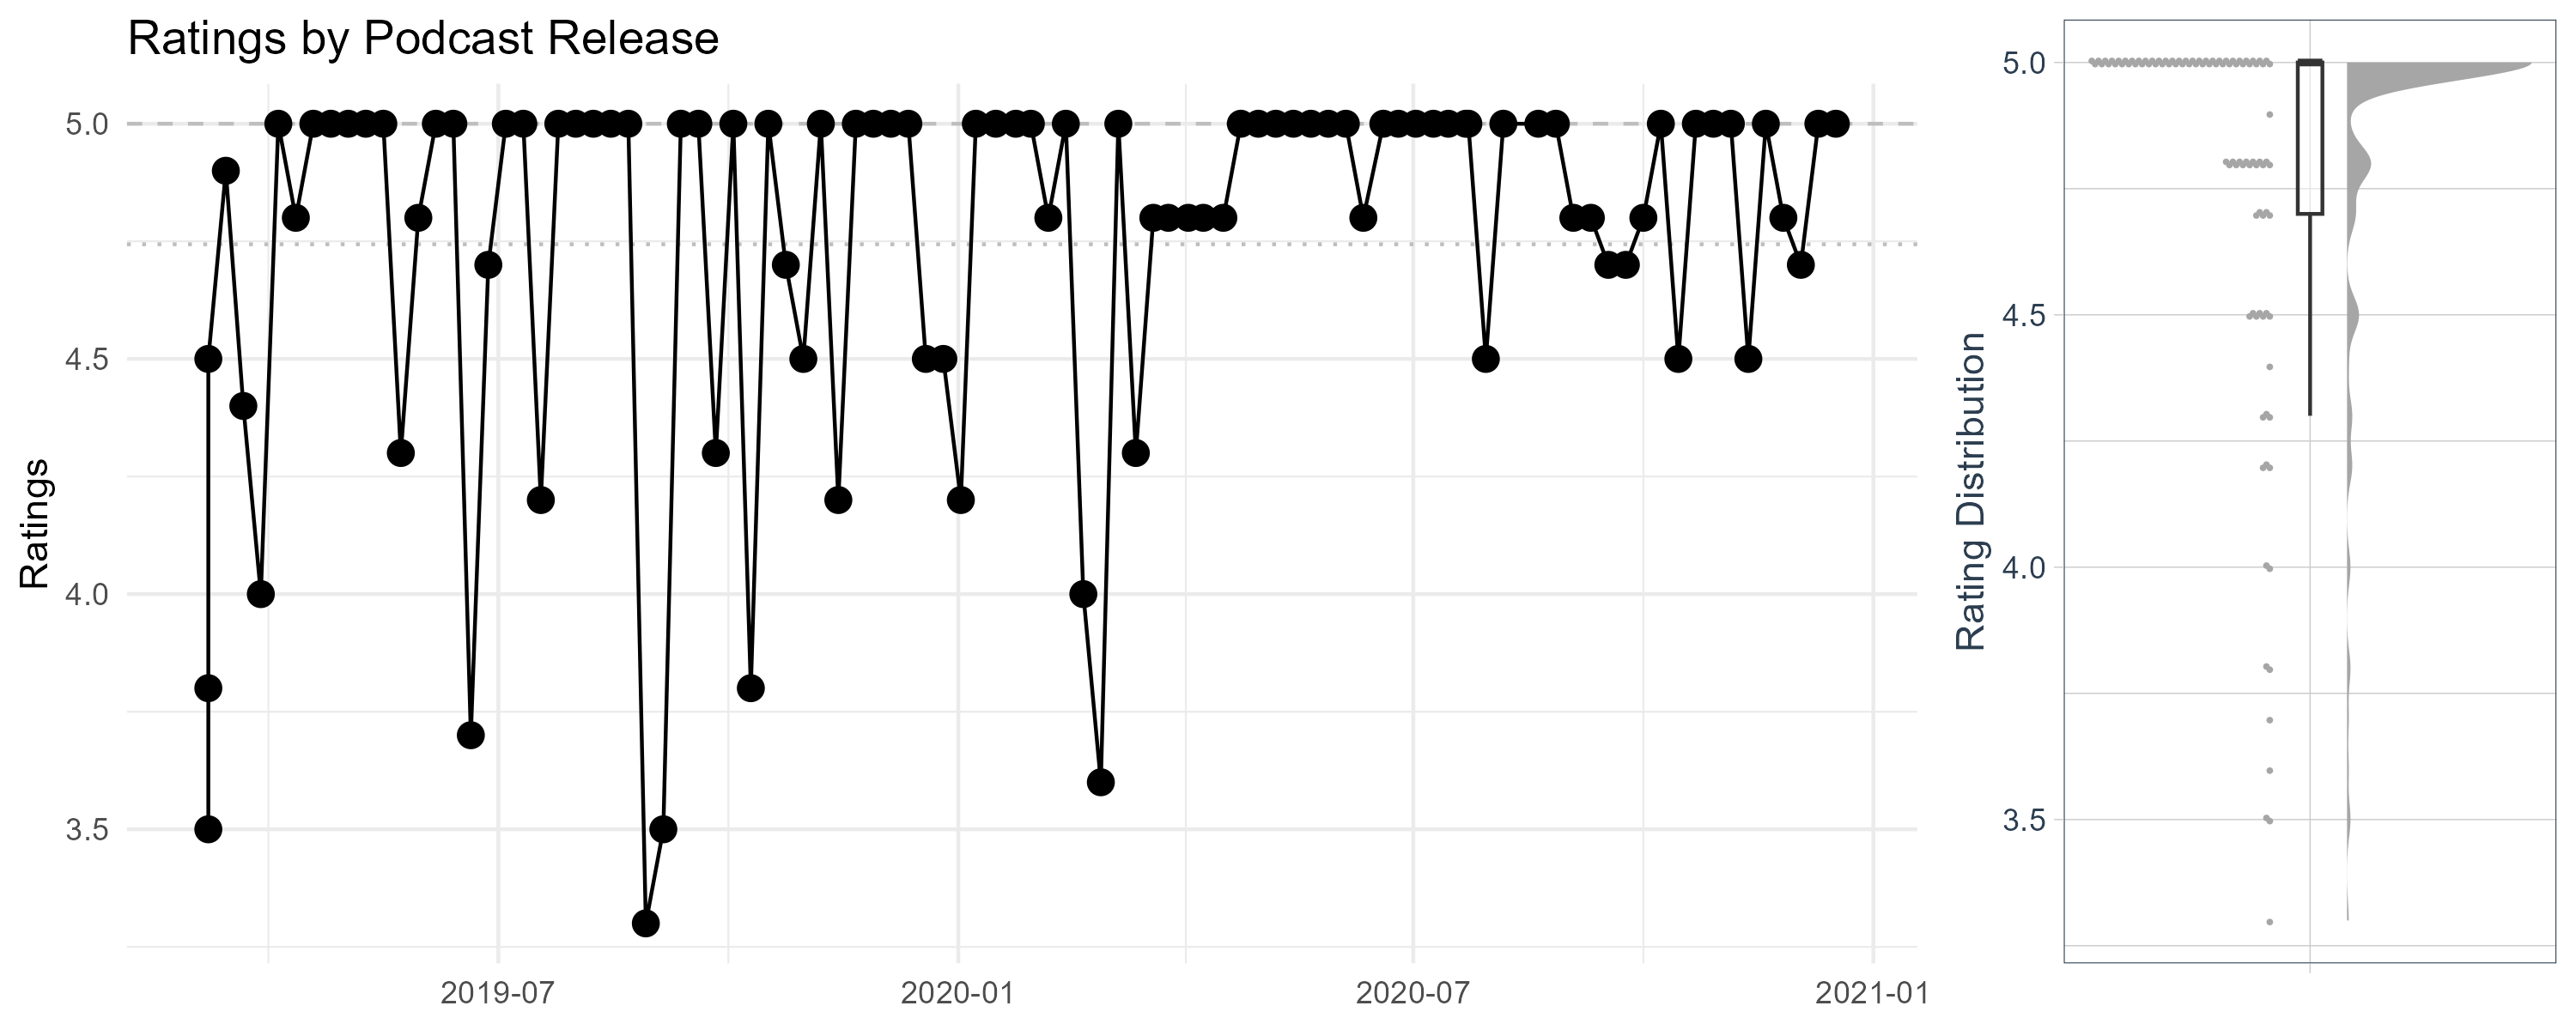
\includegraphics[width=\textwidth]{../rek-data-beers/R/figures/iskisur_ratings}
    \begin{itemize}
        \item Average rating: 4.74 out of 5
        \item 54 episodes with a perfect 5.0 score (56\% of total)
        \item Only 7 episodes with a rating below 4.0 (worst case 3.3)
    \end{itemize}
\end{frame}

\begin{frame}{Podcast on Storytel: Low Reviews}
\note{\scriptsize

Alright, let's ground ourselves with a touch of humility here.
    Taking a look at this chart, we can see a humbling snapshot: our review count isn't quite as jaw-dropping as we might have hoped.
    Sure, we've got a commendable rating, but in terms of review numbers?
    Our 444 reviews are dwarfed by the 25,627 the audiobooks received.
    Clearly, we were a small fish in the Storytel pond.

    \emph{Full disclosure}: I didn't religiously review our podcast episodes.
    After the initial rush of hearing our voices on the platform, I realized that since I was relistening during post-processing
    (penning the accompanied text summaries – a must-read, by the way), there wasn't much point in re-re-relistening.
    I've believe my co-hosts shared my sentiment.

    However, every silver lining has its cloud:
    \begin{itemize}
        \item We always had at least \emph{one} die-hard fan who never failed to review,
        \item and we'll forever be grateful to those \emph{four} mainstays who consistently showered us with feedback.
    \end{itemize}

    While our podcast felt like a cozy book club, a running joke was that there was only one listener.
    But looking at our review count, it seems the joke was closer to the truth than we thought.
    Nonetheless, it's not the quantity that matters, but the quality.

}
    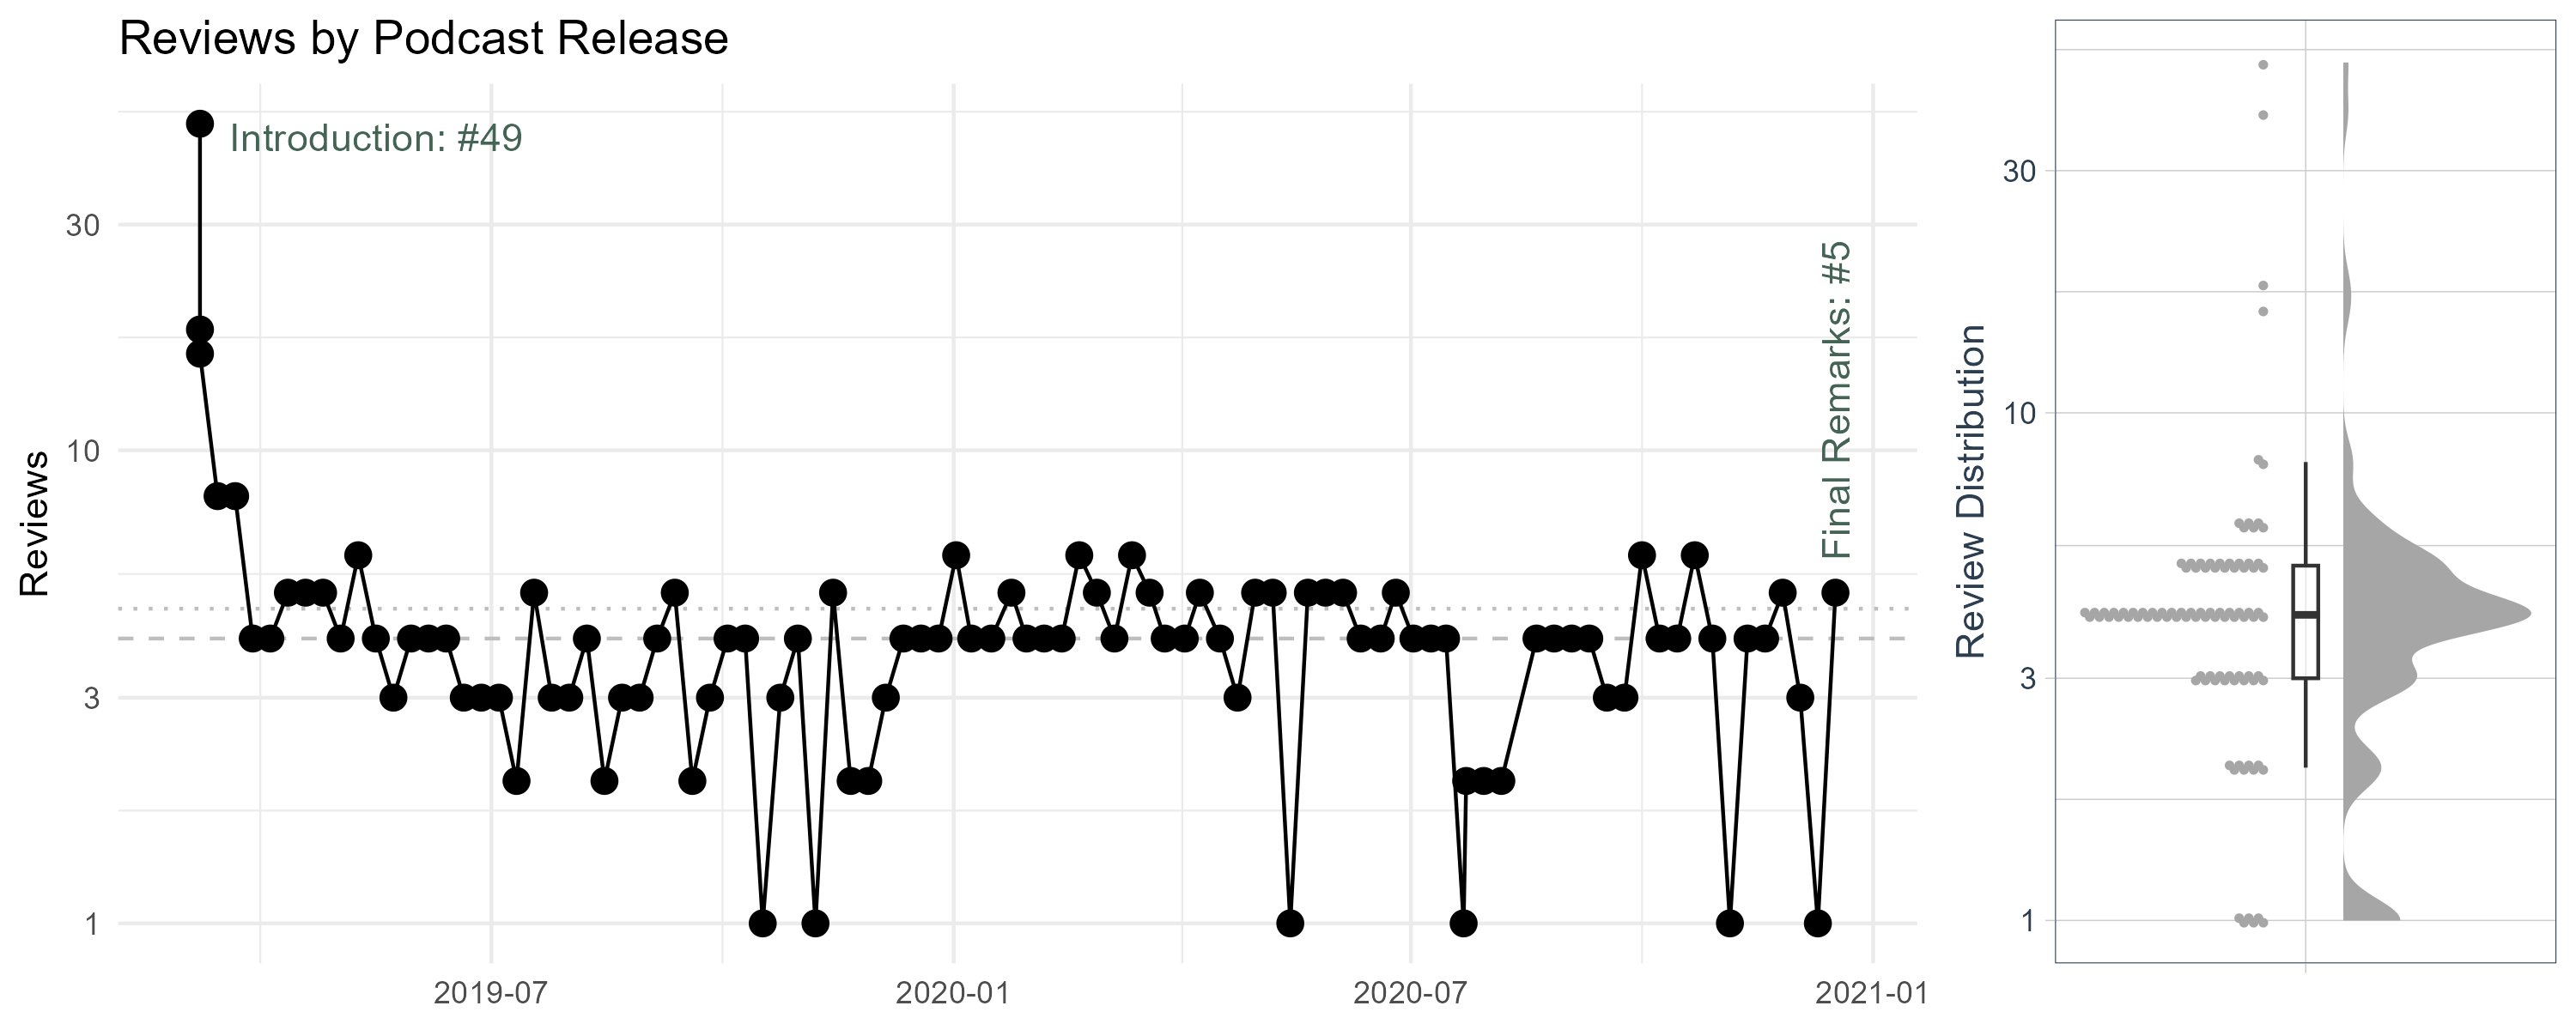
\includegraphics[width=\textwidth]{../rek-data-beers/R/figures/iskisur_reviews}
    \begin{itemize}
        \item Number of reviews: 444 total (25,627 for the audiobooks)
        \item At least one active fan throughout the period
        \item Four regular fans who consistently provided review
    \end{itemize}
\end{frame}

\begin{frame}{Podcast Platform Comparison}
    \note{
    As we conclude, here's a bird's-eye view of our podcast journey:
    \begin{itemize}
        \item We went from crafting 46 episodes on Alvarpið to a staggering 96 on Storytel.

        \item The average episode length slightly increased on Storytel.

        \item Notice the stark difference in release consistency: Alvarpið saw gaps as long as 161 days, while Storytel never went beyond a 14-day hiatus.

        \item In terms of overall engagement, both platforms gave us roughly 20 months of active podcasting each, but let's not forget that 4.1-month pause we took in between.
    \end{itemize}

    Most importantly, we had a blast throughout the journey, and we managed to cover all 47 books in the series in record time (in true Margit fashion)
    }
    \begin{table}[]
        \begin{tabular}{l|rr|rr|rrr|r}
            & \rotatebox{90}{Episodes} & \rotatebox{90}{Books} &
            \rotatebox{90}{Total Running Time (hours)} & \rotatebox{90}{Average Length (min)} &
            \rotatebox{90}{Median Days to Next}
            & \rotatebox{90}{Average Days to Next}  & \rotatebox{90}{Max Days to Next}  &
            \rotatebox{90}{Months Active} \\
            \midrule
            Alvarpið & 46  & 6  & 37.2  & 48.50 & 7 & 13.69 & 161 & 20.3  \\
            Storytel & 96  & 47 & 92.2  & 57.61 & 7 & 6.85  & 14  & 21.4  \\
            \midrule
            & 142 &    & 129.4 &       &   &       &     & 45.8*
        \end{tabular}
    \end{table}

    \vfill
    \footnotesize{*4.1 months hiatus between Alvarpið and Storytel}
\end{frame}
